\documentclass[aspectratio=169]{beamer}
\usepackage[utf8]{inputenc}


\usetheme{Madrid}
\usecolortheme{default}
\useinnertheme{circles}

\definecolor{Logo1}{rgb}{0.06274509803921569, 0.17254901960784313, 0.32941176470588235} %(16, 44, 84)
\definecolor{Logo2}{rgb}{1.0, 0.5764705882352941, 0.3254901960784314} %(255, 147, 83)

\setbeamercolor*{palette primary}{bg=Logo1, fg=white}
\setbeamercolor*{palette secondary}{bg=Logo2, fg=white}
\setbeamercolor*{palette tertiary}{bg=white, fg=Logo1}
\setbeamercolor*{palette quaternary}{bg=Logo1,fg=white}
\setbeamercolor{structure}{fg=Logo1} % itemize, enumerate, etc
\setbeamercolor{section in toc}{fg=Logo1} % TOC sections

%------------------------------------------------------------








%------------------------------------------------------------
%This block of code defines the information to appear in the
%Title page
\title[PAVIC] %optional
{Correção de mapas de profundidade através de técnica de inpainting}

%\subtitle{And its subtitle}

\author[Gustavo Castro] % (optional)
{Gustavo Moreira Oliveira de Castro}

\institute[UFAC] % (optional)
{
  Programa de Pós Graduação em Ciência da Computação\\
  Universidade Federal do Acre
}

\date[PPGCC] % (optional)
{Apresentação de pesquisa}


\logo{
\includegraphics[height=.6cm]{ourlogo.png}}

%End of title page configuration block
%------------------------------------------------------------





%------------------------------------------------------------
%The next block of commands puts the table of contents at the 
%beginning of each section and highlights the current section:

\AtBeginSection[]
{
  \begin{frame}
    \frametitle{Table of Contents}
    \tableofcontents[currentsection]
  \end{frame}
}
%------------------------------------------------------------


\begin{document}

%The next statement creates the title page.
\frame{\titlepage}


%---------------------------------------------------------
%This block of code is for the table of contents after
%the title page
\begin{frame}
\frametitle{Table of Contents}
\tableofcontents
\end{frame}
%---------------------------------------------------------


\section{Introdução}

%---------------------------------------------------------
%Changing visivility of the text
\begin{frame}
\frametitle{Contextualização da pesquisa}
A pesquisa a ser desenvolvida tem como base a correção de mapas de profundidade obtidos por sensores RGB-D e câmeras ToF utilizando algoritmos de inpainting aliados à correção guiada e não guiada. 
\begin{columns}
    \column{0.5\textwidth}
    \begin{itemize}
    \item Mapas de profundidades são imagens em que o valor dos pixels é diretamente relacionado à distância do objeto ao sensor de captura
    \item Sensores comuns de profundidade possuem alta confiabilidade nos pixels adquiridos, mas também produzem leituras inválidas.
    \item O problema de correção de mapas de profundidade implica em realizar novas predições somente nos pixels que o sensor considerou como inválidos.
\end{itemize}

    \column{0.5\textwidth}

    \begin{figure}
        \centering
        \includegraphics[width=\textwidth]{figs/depth_problema.png}
        \caption{Exemplo de mapa de profundidade com defeitos.}
        \label{fig:enter-label}
    \end{figure}
\end{columns}


\end{frame}

\begin{frame}{Tecnologias comuns em mapas de profundidade}
    \begin{figure}
        \centering
        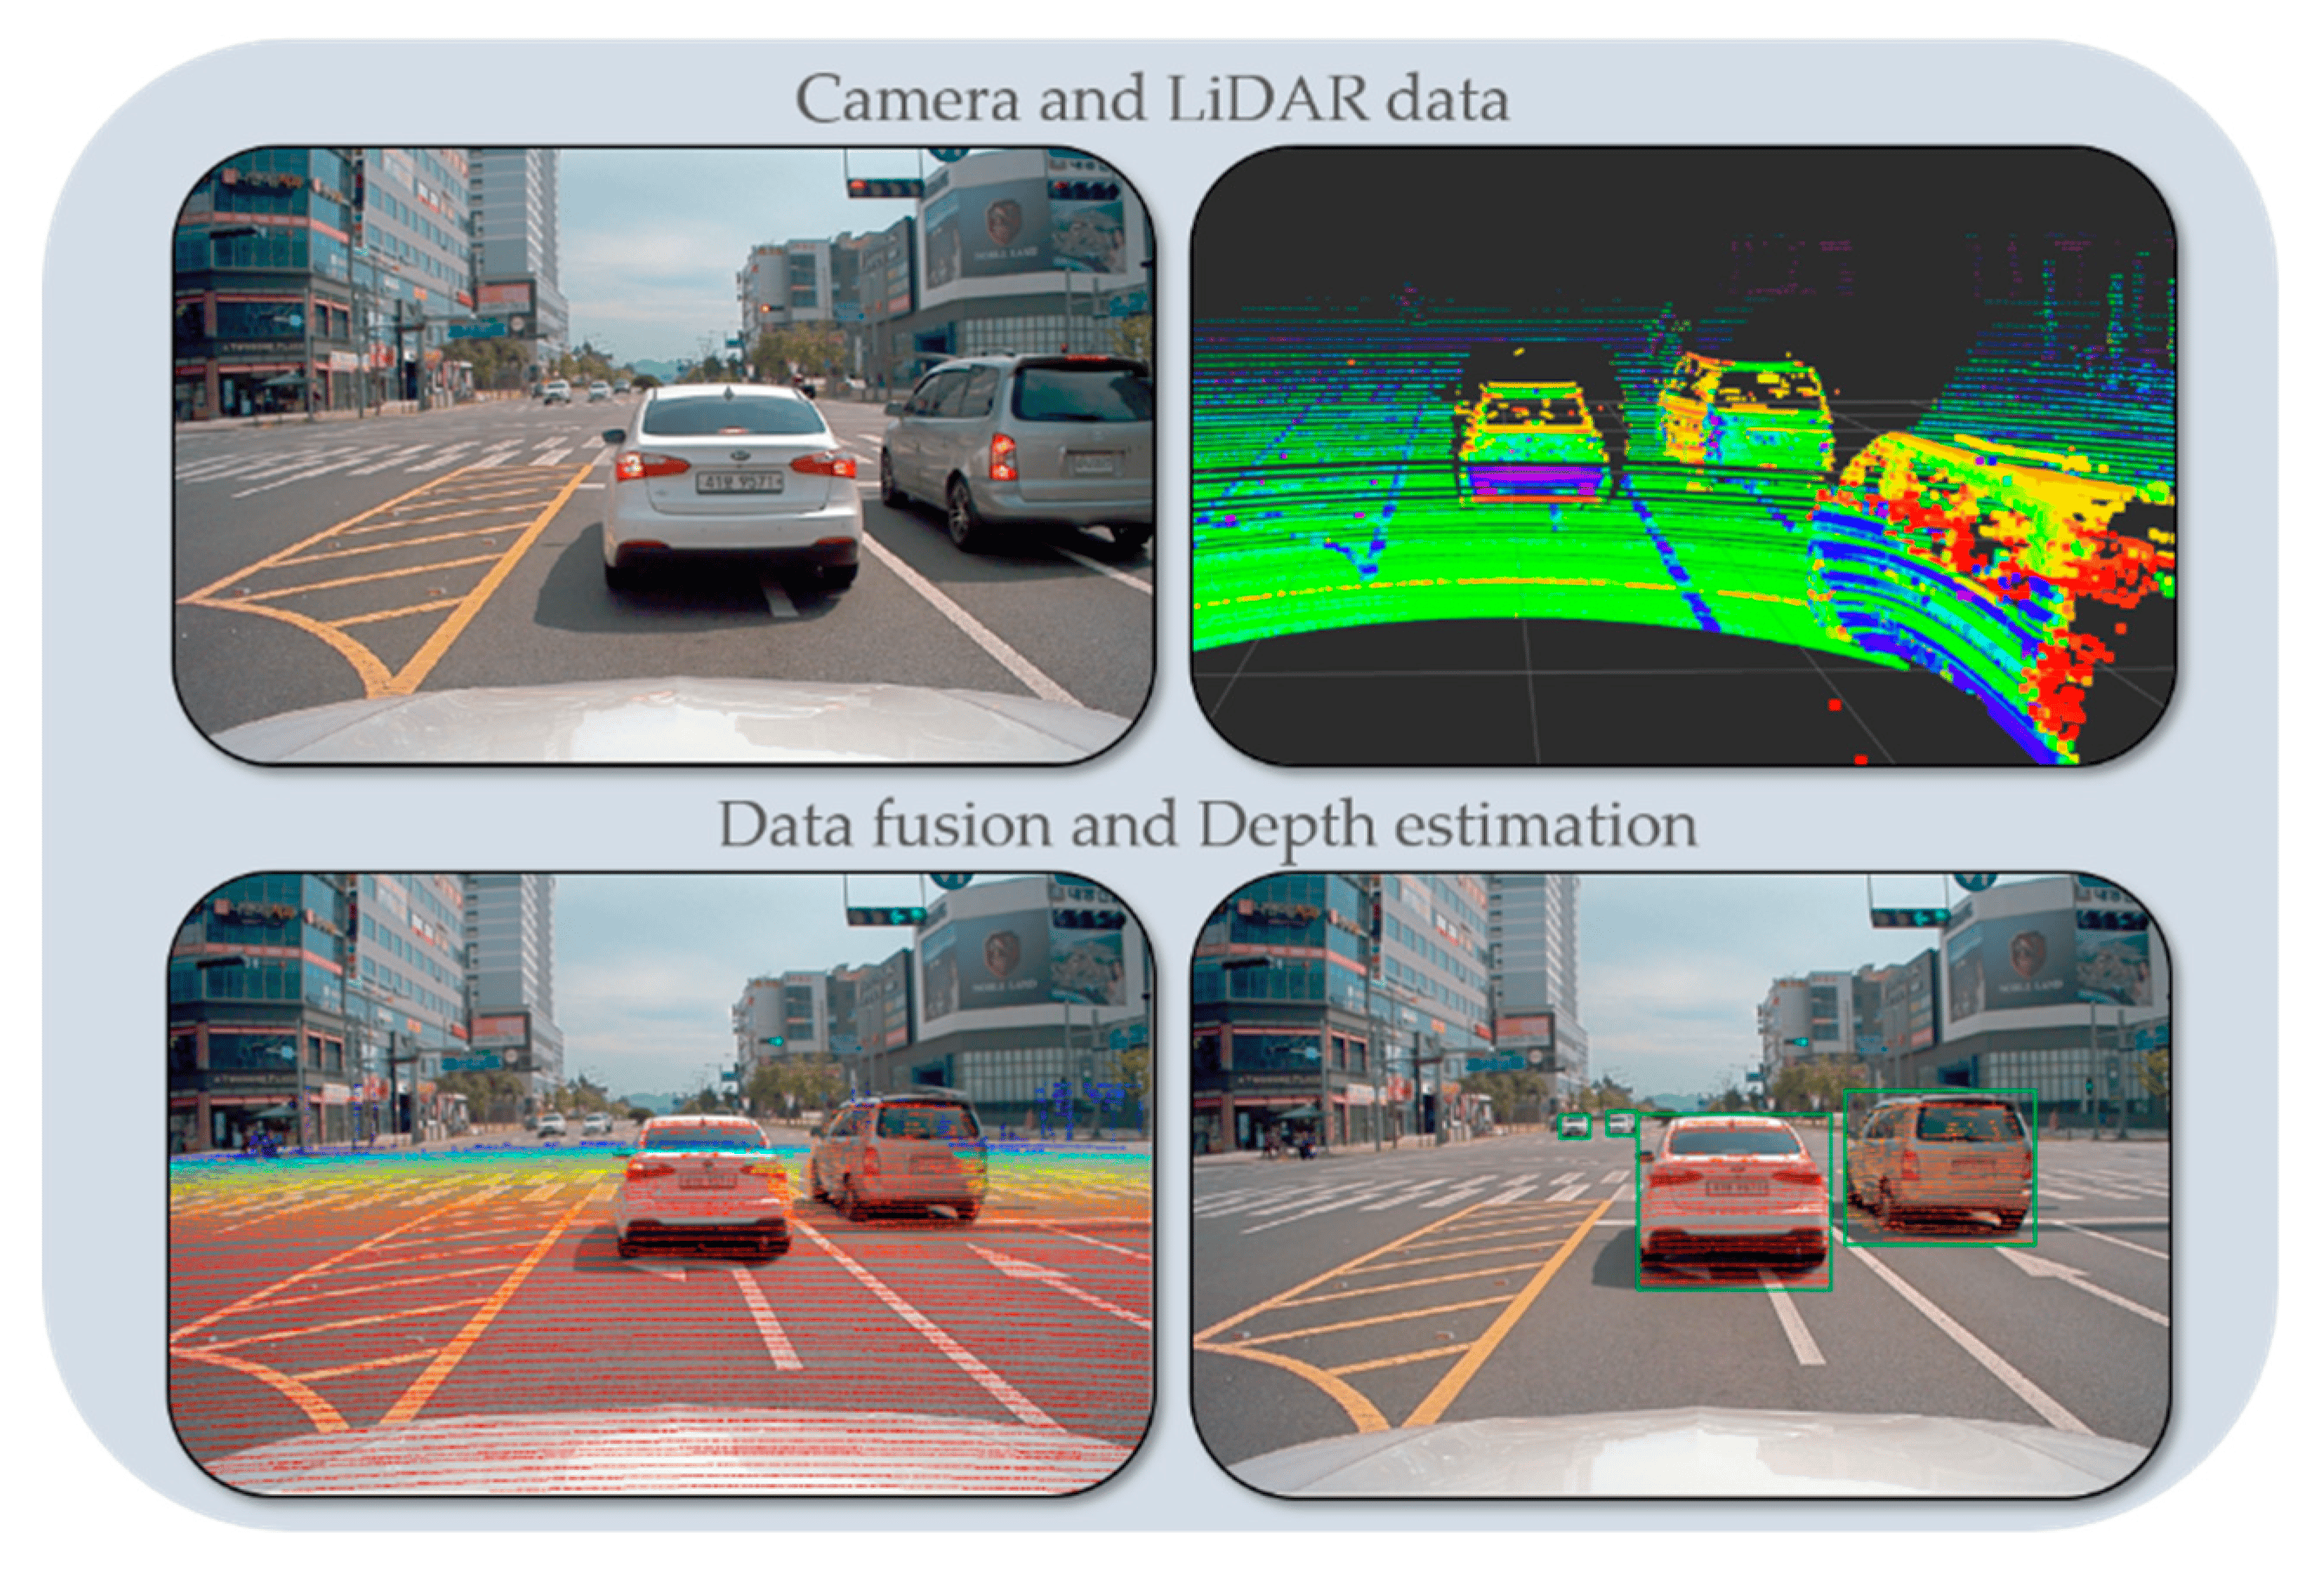
\includegraphics[scale=.1]{figs/lidar.png}
        \caption{Imagens de LiDAR}
        \label{fig:enter-label}
    \end{figure}
\end{frame}

\begin{frame}{Tecnologias comuns de mapas de profundidade}
    \begin{figure}
        \centering
        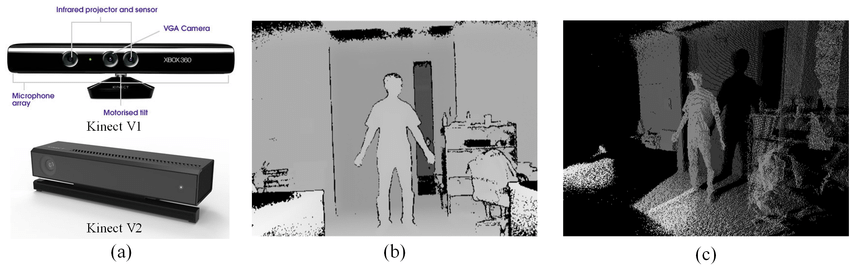
\includegraphics[width=\textwidth]{figs/a-Kinect-sensors-8-9-b-The-25D-depth-map-captured-by-Kinect-V2-c-The.png}
        \caption{Xbox kinect}
        \label{fig:enter-label}
    \end{figure}
\end{frame}

\begin{frame}{Tecnologias comuns de mapas de profundidade}
    \begin{figure}
        \centering
        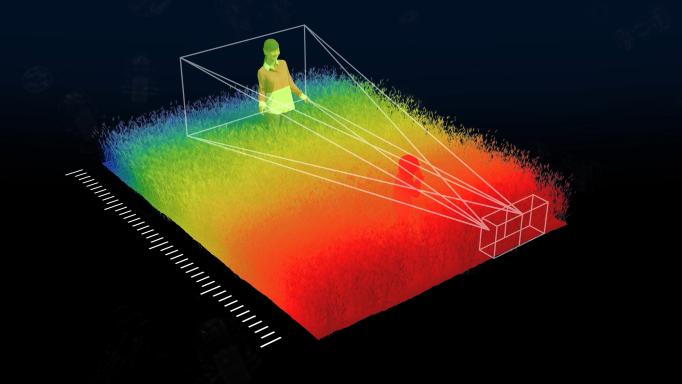
\includegraphics[width=.7\textwidth]{figs/CP_DM_SI_CR.png}
        \caption{Stereo Vision Depth Estimation}
        \label{fig:enter-label}
    \end{figure}
\end{frame}
%---------------------------------------------------------


%---------------------------------------------------------
%Example of the \pause command
\begin{frame}{Mapas de profundidade}

\begin{figure}
    \centering
    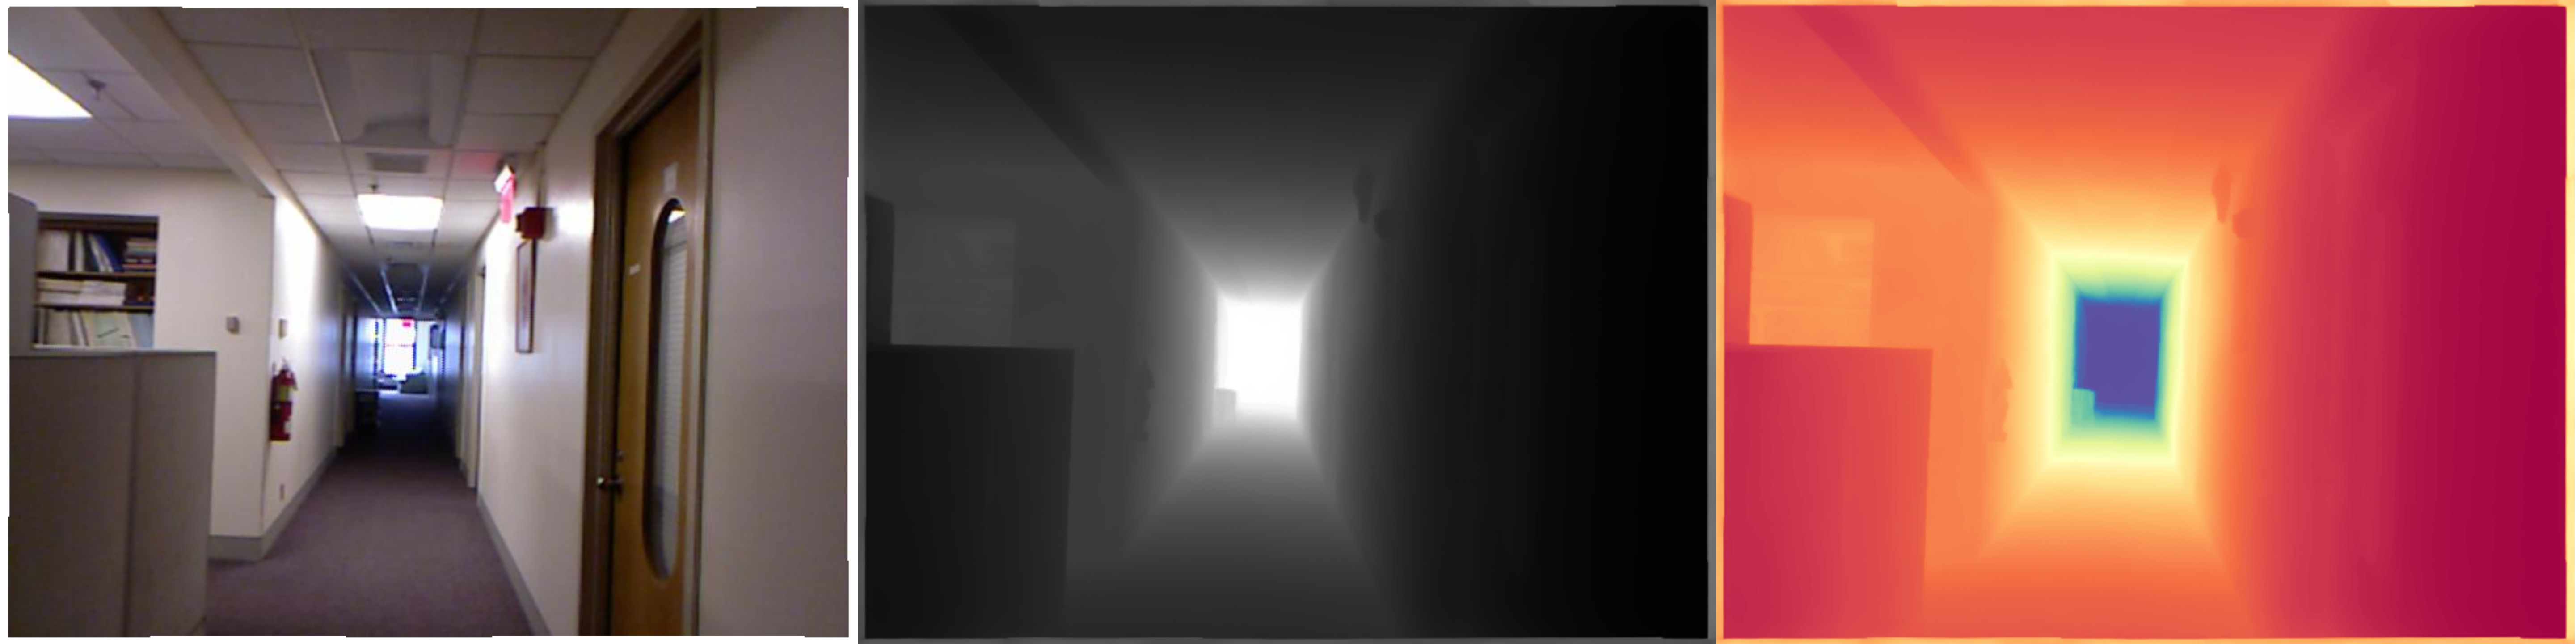
\includegraphics[width=\textwidth]{figs/example_depth.png}
    \caption{Exemplo de mapa de profundidade (Dataset NYU Depth V2)}
    \label{fig:enter-label}
\end{figure}
\end{frame}

\begin{frame}{Mapas de profundidade}

\begin{figure}
    \centering
    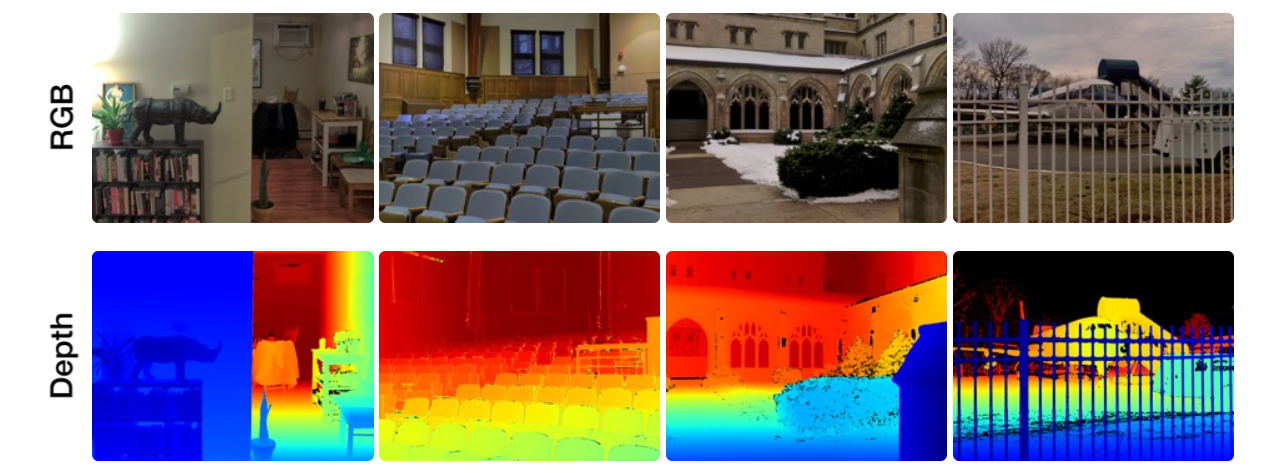
\includegraphics[width=\textwidth]{figs/exemplo1.png}
    \caption{Exemplo de mapa de profundidade (DIODE Dataset)}
    \label{fig:enter-label}
\end{figure}
\end{frame}


\begin{frame}{Mapas de profundidade com erros}

\begin{figure}
    \centering
    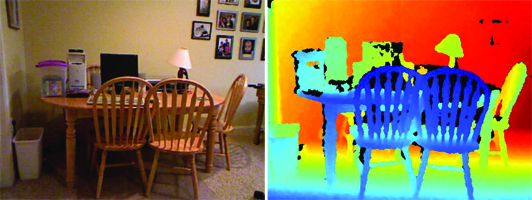
\includegraphics[scale=2]{figs/nyu_depth_v2_raw.jpg}
    \caption{Exemplo de mapa de profundidade (Dataset NYU Depth V2)}
    \label{fig:enter-label}
\end{figure}
\end{frame}
%---------------------------------------------------------

\section{Objetivos}

\begin{frame}{Objetivos}

Este trabalho possui como objetivo geral realizar a correção de mapas de profundidade com erros através de redes neurais artificiais e técnicas de \textit{inpainting}.

\begin{itemize}
    \item Realizar revisão de literatura de métodos de correção de mapas de profundidade.
    \item Escolher um método de \textit{inpainting} baseado em redes neurais artificiais.
    \item Estabelecer um método de geração de máscaras de erro para treinamento.
    \item Corrigir mapas de profundidade com algoritmo de \textit{inpainting} baseado em correção não-guiada.
    \item Corrigir mapas de profundidade com algoritmo de \textit{inpainting} baseado em correção guiada.
    \item Corrigir mapas de profundidade utilizando abordagem morfológica.
    \item Comparar as diferentes abordagens através de métricas de avaliação perante a diferentes níveis de pixels inválidos.
    
\end{itemize}

\end{frame}
\section{Metodologia}

%---------------------------------------------------------
%Highlighting text

\begin{frame}{Técnica de inpainting}
\begin{figure}
    \centering
    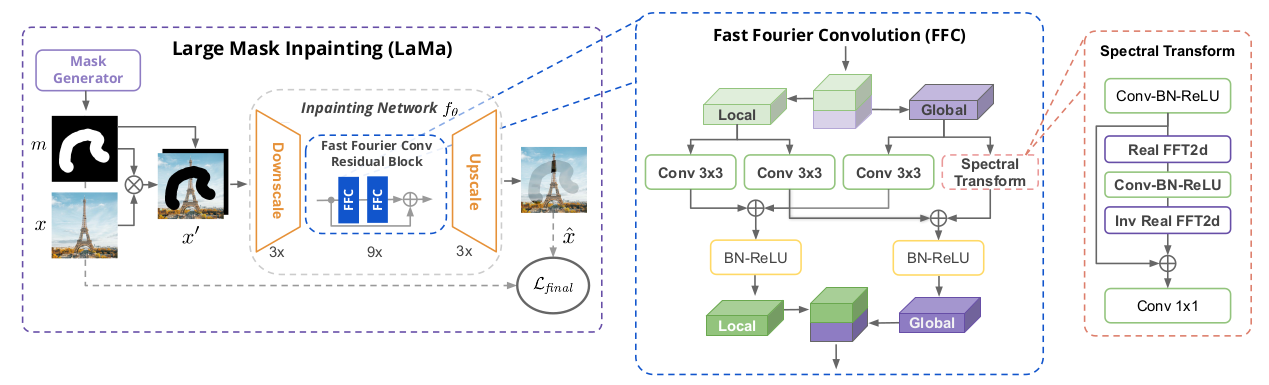
\includegraphics[width=\textwidth]{figs/lama.png}
    \caption{Esquema da técnica Lama (Large Mask inpainting)}
    \label{fig:enter-label}
\end{figure}
    
\end{frame}

\begin{frame}{Técnica de inpainting}
    \begin{figure}
        \centering
        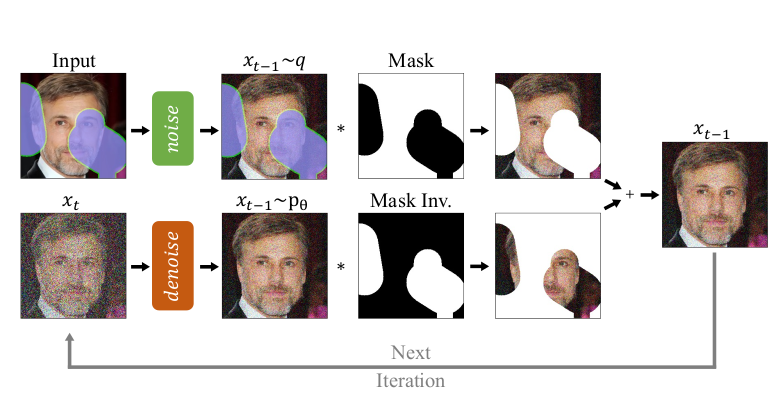
\includegraphics[width=.8\textwidth]{figs/repaint.png}
        \caption{Esquema da técnica Repaint}
    \end{figure}
\end{frame}

\begin{frame}{Técnica de inpainting}
    \begin{figure}
        \centering
        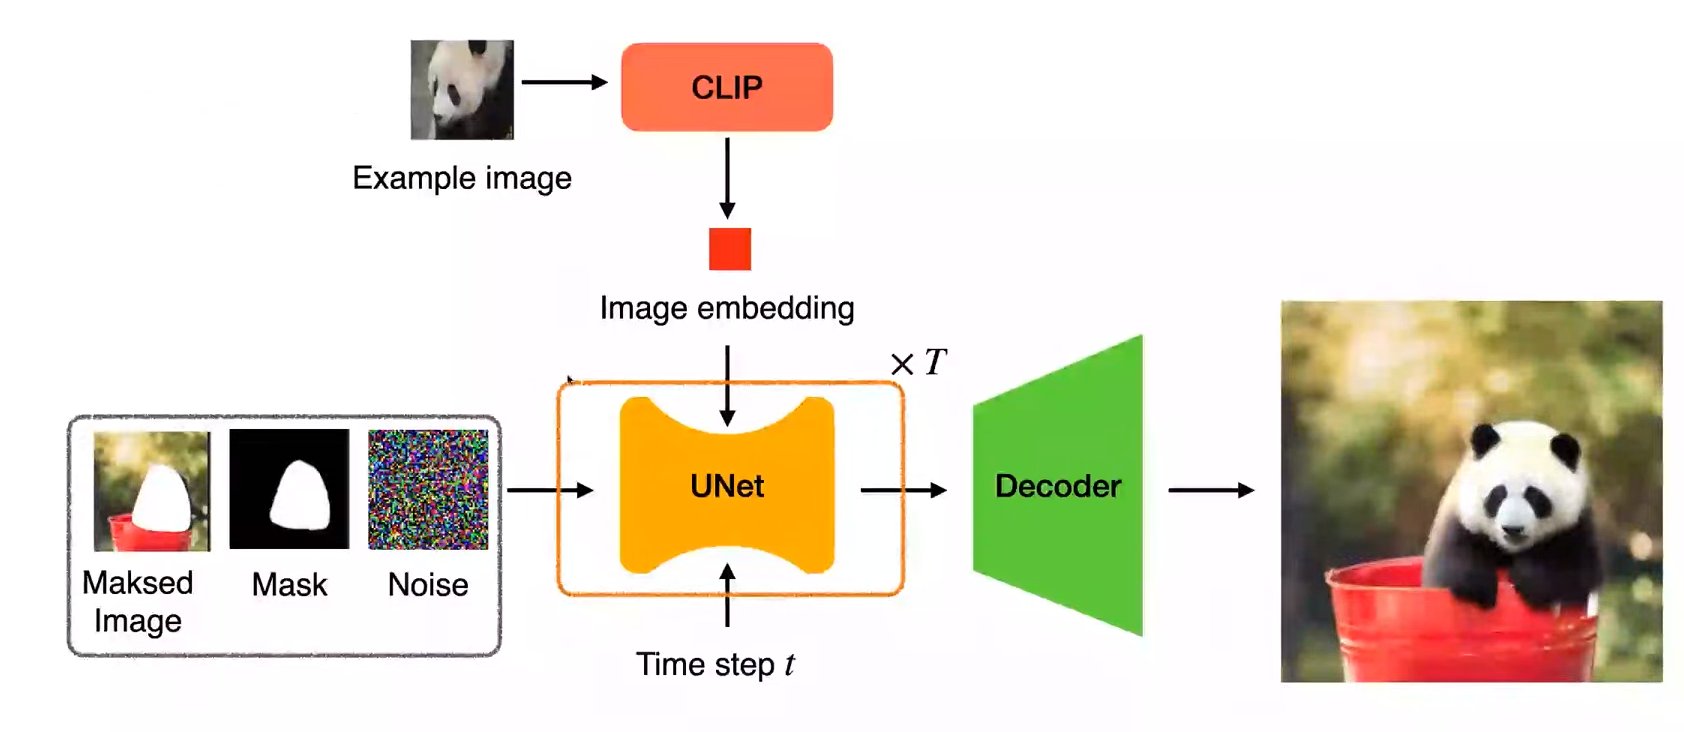
\includegraphics[width=\textwidth]{figs/paint_by_example.png}
        \caption{Esquema da técnica Paint by example}
    \end{figure}
\end{frame}


\begin{frame}{Categorias de correção}

Para a tarefa de correção de mapas de profundidade utilizando redes neurais, há duas categorias principais que se diferenciam pelos dados utilizados:

\begin{itemize}
    \item \textbf{Correção não-guiada}: Objetiva completar diretamente as partes faltantes utilizando como entrada somente o mapa de profundidade
    \item \textbf{Correção guiada}: Objetiva completar as partes faltantes utilizando como entrada tanto o mapa de profundidade quanto a imagem RGB correspondente.
\end{itemize}
\end{frame}

\begin{frame}{Categorias de correção}

Entre os métodos de correção guiada, ainda destacam-se:

\begin{itemize}
    \item \textbf{Early Fusion}: A imagem RGB é concatenada ao mapa de profundidade e o conjunto é utilizado como entrada da rede neural
    \item \textbf{Late Fusion}: A informação RGB é adicionada como contexto na arquitetura da rede através de outro ramo
\end{itemize}
    
\end{frame}

\begin{frame}{Categorias de correção}

\begin{figure}
    \centering
    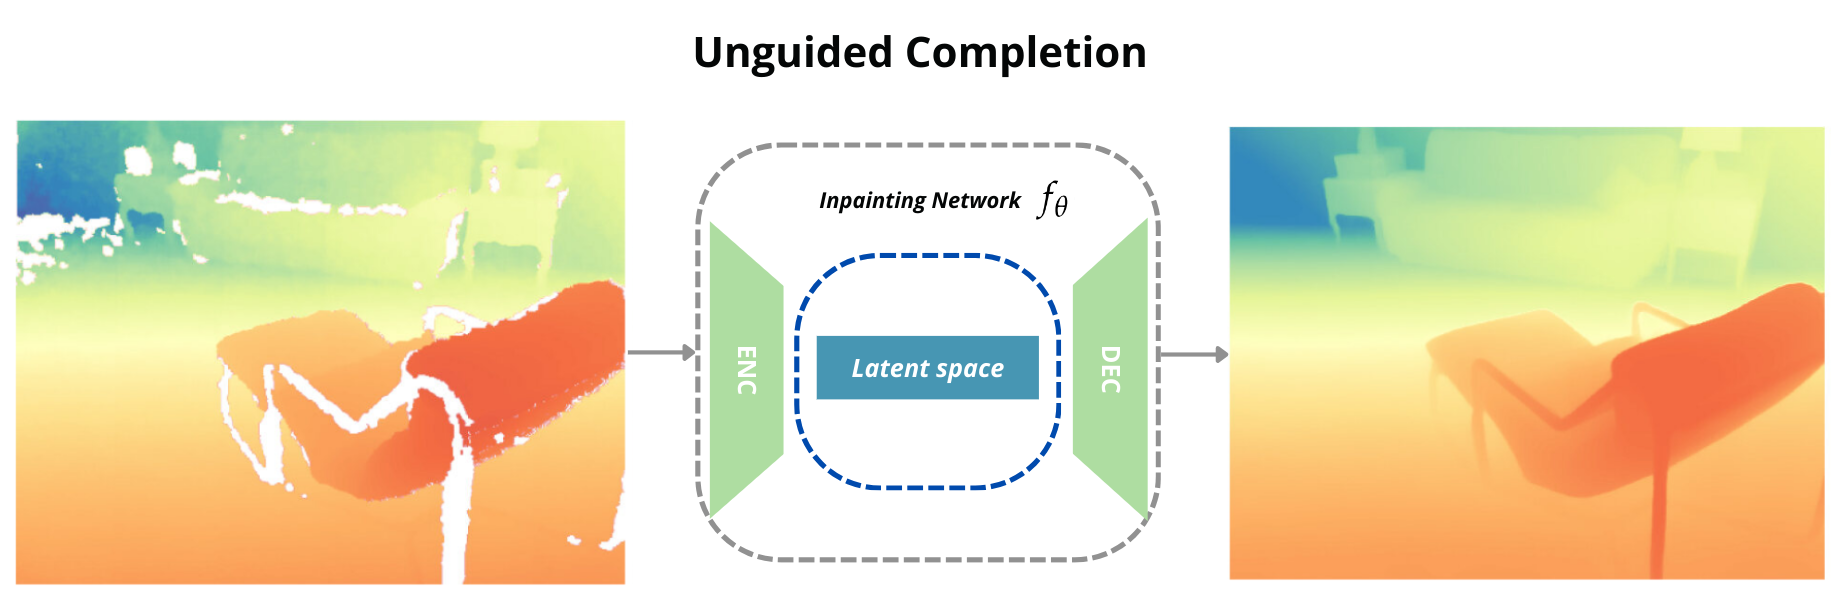
\includegraphics[width=\textwidth]{figs/unguided1.png}
    \caption{Esquema de correção não-guiada}
    \label{fig:enter-label}
\end{figure}
    
\end{frame}

\begin{frame}{Categorias de correção}

\begin{figure}
    \centering
    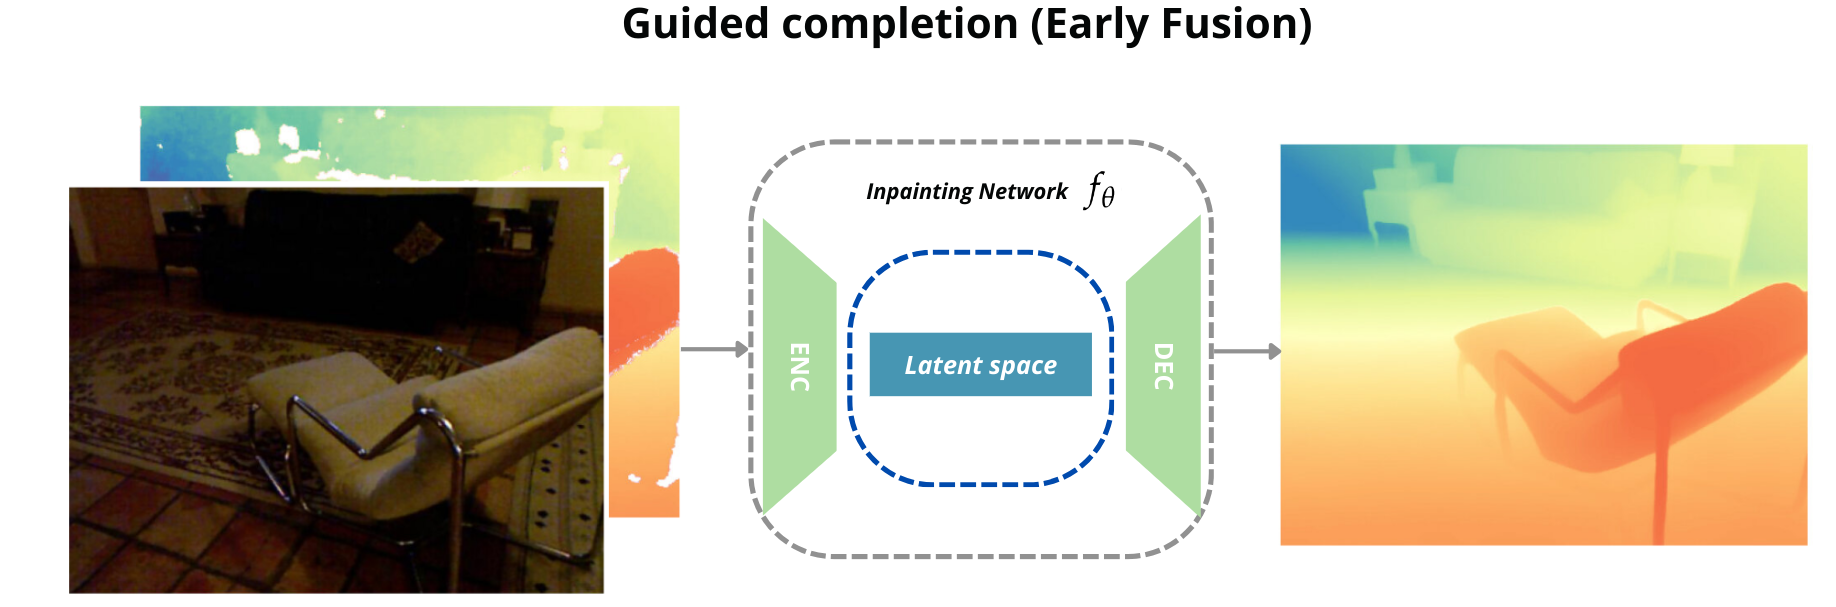
\includegraphics[width=\textwidth]{figs/earlyfusion1.png}
    \caption{Esquema de correção guiada com early fusion}
    \label{fig:enter-label}
\end{figure}
    
\end{frame}

\begin{frame}{Categorias de correção}

\begin{figure}
    \centering
    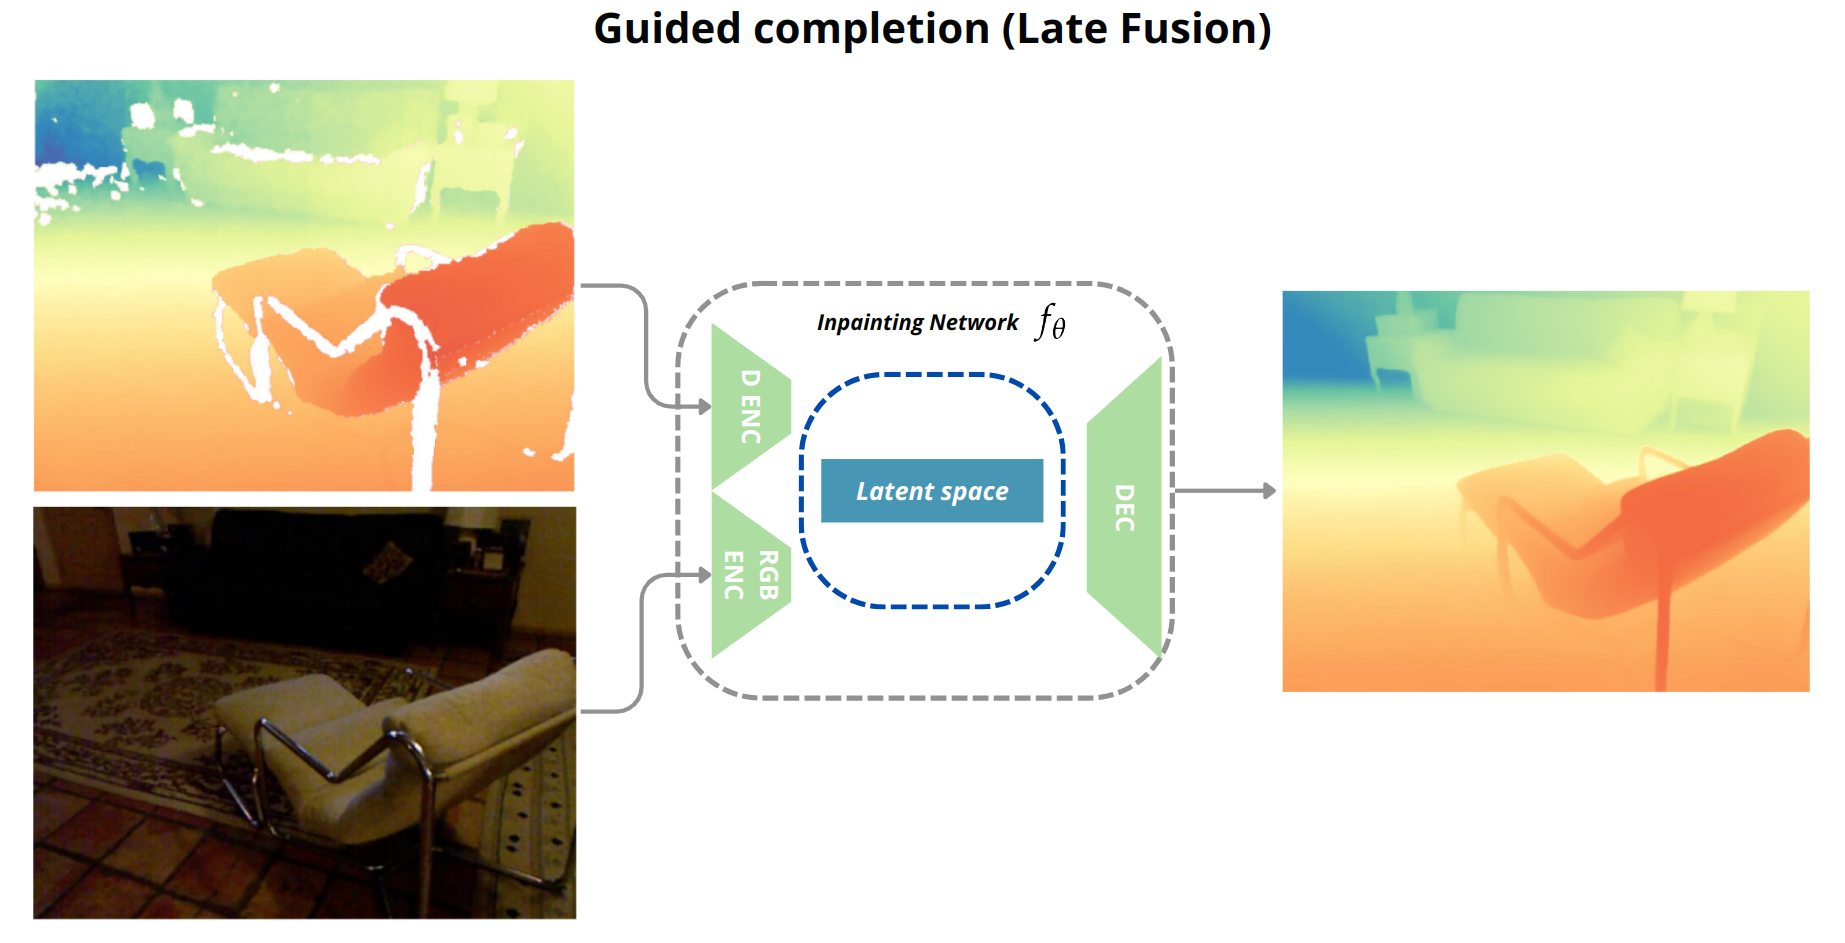
\includegraphics[width=\textwidth]{figs/latefusion1.png}
    \caption{Esquema de correção guiada com late fusion}
    \label{fig:enter-label}
\end{figure}
    
\end{frame}




\begin{frame}{Datasets}

\begin{itemize}
    \item \textbf{Hypersim}: Cenas virtuais fotorrealísticas renderizadas. Contendo 77400 imagens com RGB e depth ground truth 
    \item \textbf{MatterPort3D}: Dataset com vistas panorâmicas e 194400 imagens RGB e raw depth. Depth ground truth pode ser calculado. 
    \item \textbf{Nyu Depth V2}: Cenas internas capturadas com câmeras RGB-D, cerca de 40000 pares de RGB e depth ground truth.
\end{itemize}
    
\end{frame}




\begin{frame}{Métricas}

 
   $$ Abs Rel = \frac{1}{N} \sum_{i}^{N} \left |  d_i - \hat{d_i}\right | / \hat{d_i}$$
   $$ \delta_Z = max (\frac{d_i}{\hat{d_i}} , \frac{\hat{d_i}}{d_i}) < 1.25^Z $$
   $$ RMSE = \sqrt{\sum_{i=1}^{n}\frac{(y_i - \hat{y_i})^2}{n}}$$

\end{frame}


\begin{frame}{Resumo das atividades}
    \begin{itemize}
        \item Foco na escrita do documento de qualificação
        \item Dúvidas em relação ao experimento
        \item Problemas em relação aos dados
        \item Nova técnica para depth inpainting com fusão tardia (Paint by Example)
        \item Foi investigada a possibilidade de utilizar transformers
        \item Iniciou um estudo mais aprofundado de modelos de difusão
    \end{itemize}
\end{frame}

\begin{frame}{Metas}
    \begin{block}{Curto prazo}

\begin{itemize}
    \item Escrever documento de qualificação: Introdução, trabalhos relacionados, problemática, metodologia, cronograma
    \item Treinar o Lama para reconstruir mapas de profundidade com o dataset Hypersim
    \item Montar o laboratório de métricas para reconstrução
\end{itemize}


\end{block}

    \begin{block}{Médio prazo}
\begin{itemize}
    \item Treinar o guided diffusion (Repaint) para construir mapas de profundidade
    \item Codar o experimento do paint by example
    \item Estudar o encoder CLIP com o objetivo de modifica-lo
    \end{itemize}
\end{block}

\end{frame}

%---------------------------------------------------------


\end{document}